\documentclass[12pt,onecolumn,notitlepage]{article}
\usepackage[letterpaper,vmargin={1in,1in},hmargin={1in,1in}]{geometry}
\usepackage{graphicx}
\usepackage{cite}
\usepackage[small]{caption}
\let\endtitlepage\relax
\def\thesection{\arabic{section}. \normalsize}
\title{\vspace{-4ex} \textbf{Group 2 Project Proposal}}
\author{Zachary Estrada \and Chandini Jain \and Jonathan Lai}

\begin{document}
\maketitle

%%%Thinking of removing abstract
\textbf{Abstract:} Group 2 proposes to study the convergence
properties of simulated annealing, genetic algorithms, and ant-colony approaches towards
finding optimal solutions for various travelling salesman problems.  Code will be tested
to find convergence rate, wall-clock time, and for solution space exploration.  For future studies,
we will consider looking at parallel and/or GPU solutions to accelerate algorithms.

\section{Introduction}
\begin{figure}
\centering
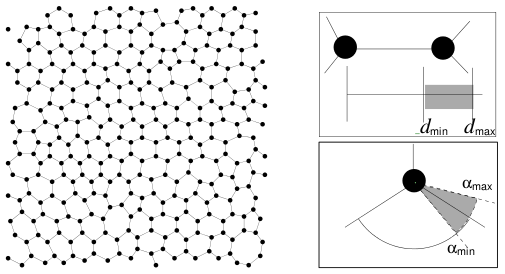
\includegraphics[width=0.75\textwidth]{Figures/amorphousSilicon.png}
\caption{An example of an amorphous solid under simulation.  A maximum vertex number of 3 is defined, along with minimum and maximum angles and bond lengths; taken from: Ref. \protect\citenum{Peinado1997gwt}}
\label{fig:amorphousSilicon}
\end{figure}


\section{Simulated Annealing}
Simulated annealing is a stochastic approach towards minimizing an energy function.

\section{Genetic Algorithms}
Unlike simulated annealing, genetic algorithms rely on a population approach to 

\section{Ant-Colony Approaches}
Ant Colony Optimization\cite{Dorigo96theant} draws inspiration from the behavior of ants as they develop a path from their nest to a food source.  As ants travel, they deposit pheromones.  These pheromones can be detected by other ants and the ants are more likely to follow a path with higher pheromone concentration.  In addition to the ants depositing pheromones, these pheromones will evaporate over time.  This means that shorter paths will allow larger pheromone concentrations to buildup as ants will be depositing pheromones quicker than they evaporate.  Eventually, the system will converge on a minimum solution.  A global minimum is pursued by starting out with a large number of ants and by tuning the weight at which pheromones influence decisions. 

\section{Go with the Winner Approaches}
Simulated annealing probabilistically convergences to the optimal solution at the rate
 of $O(\frac{1}{n})$ where n is the number of independent runs.  
Using heuristic schemes such as the ``Go with the Winner''~\cite{Aldous1994gwt}, hereby referred to as GWW, 
one can improve this convergence rate to $O(log \frac{1}{n})$ and have recently found their way into molecular modeling applications~\cite{Peinado1997gwt}.  In general terms, the GWW algorithm mirrors that of simulated annealing; however, each independent run is periodically reassessed to determine if one is converging upon a losing solution.  Runs with 
no chance for success are immediately discarded while runs with the best chance of finding an optimal solution
are replicated; thus, GWW generates an ensemble of independent runs filled with  ``winners''.  

\section{Analysis}
To assess the performance of our optimization schemes, we would


\bibliographystyle{plain}
\bibliography{AtomicScaleProposal}
\end{document}
